\documentclass[10pt]{article}

\usepackage[a4paper,margin=2.25cm]{geometry}
\usepackage[T1]{fontenc}
\usepackage[utf8]{inputenc}
\usepackage{lmodern}
\usepackage{microtype}
\usepackage{booktabs}
\usepackage{tabularx}
\usepackage{longtable}
\usepackage{array}
\usepackage{graphicx}
\usepackage{xcolor}
\usepackage{hyperref}
\usepackage{enumitem}
\usepackage{fancyhdr}

\definecolor{navy}{HTML}{183153}
\definecolor{blue}{HTML}{2563EB}
\definecolor{orange}{HTML}{D97706}
\definecolor{softgray}{HTML}{F3F4F6}
\hypersetup{colorlinks=true,linkcolor=navy,citecolor=navy,urlcolor=blue}
\setlength{\parindent}{0pt}
\setlength{\parskip}{0.55em}
\setlist{nosep,leftmargin=1.5em}
\pagestyle{fancy}
\fancyhf{}
\lhead{ReAct Reproduction Study}
\rhead{HotpotQA and FEVER}
\cfoot{\thepage}
\renewcommand{\headrulewidth}{0.3pt}

\newcommand{\method}[1]{\textsc{#1}}
\newcommand{\pct}[1]{#1\%}
\newcommand{\code}[1]{\texttt{#1}}

\title{Reasoning, Acting, and Fallback:\\A Reproduction Study on HotpotQA and FEVER}
\author{ReAct ICLR 2023 Reproduction Project}
\date{September 2026}

\begin{document}
\maketitle

\begin{abstract}
We evaluate seven prompting and agent strategies on matched 500-example subsets of HotpotQA and FEVER using Qwen2.5-7B-Instruct. The study covers Standard prompting, chain-of-thought (CoT), self-consistent chain-of-thought (CoT-SC), Act, ReAct, and two directional hybrids. On HotpotQA, ReAct followed by CoT-SC obtains the strongest answer performance, reaching 31.4 exact match (EM) and 43.54 F1. On FEVER, the same hybrid reaches 61.6 accuracy and produces no invalid final labels. Trajectory analysis shows that completed ReAct decisions are comparatively strong, but standalone ReAct is constrained by retrieval formulation and failure to finish within the interaction budget. The contrast is particularly marked on FEVER: completed ReAct trajectories achieve 67.8 accuracy, yet 258 of 500 examples return no valid label. These results support the use of fallback policies while also showing that their effectiveness depends on direction, task structure, and the cost of the route attempted first.
\end{abstract}

\section{Introduction}

ReAct interleaves natural-language reasoning with actions in an external environment, providing a mechanism by which a language model can retrieve information and revise its reasoning as evidence arrives \cite{yao2023react}. This design is attractive for knowledge-intensive tasks because it joins parametric knowledge with explicit interaction. It also creates a control problem: a model must formulate a useful query, parse the observation, decide whether more evidence is required, and finish before its action budget is exhausted.

This report studies that trade-off on two tasks used in the original ReAct work. HotpotQA is open-ended multi-hop question answering, whereas FEVER is three-way claim verification. Although both depend on factual knowledge, their output spaces and failure modes differ. A HotpotQA system must compose an answer string after following multiple relations. A FEVER system must instead map evidence to one of 	extsc{Supports}, 	extsc{Refutes}, or 	extsc{Not Enough Info}.

All quantitative results are extracted from the benchmark artifacts currently stored in \code{outputs/hotpotqa/} and \code{outputs/fever/}. The report does not estimate missing values or merge smoke tests with full runs. The accompanying deterministic utility selects and validates runs, produces machine-readable summaries, and generates the figures used below.

\section{Background}

\subsection{ReAct}

ReAct represents each interaction as a Thought, an Action, and an environment Observation. In this implementation, the action space consists of \code{Search[query]}, \code{Lookup[term]}, and \code{Finish[answer]}. Search and Lookup observations come only from the Wikipedia environment; model-generated Observation text is stopped and deterministically truncated before action parsing.

\subsection{Chain-of-Thought}

Chain-of-thought prompting elicits an intermediate reasoning trace before a final answer \cite{wei2022cot}. It provides no external evidence in these experiments, so success depends on the model's parametric knowledge and reasoning. Standard prompting provides the corresponding direct-answer baseline.

\subsection{Self-Consistency}

Self-consistency samples multiple reasoning paths and aggregates their normalized answers \cite{wang2023selfconsistency}. The runs use 21 samples at temperature 0.7. FEVER voting occurs over three canonical labels; HotpotQA voting occurs over normalized open-ended strings, creating a much larger answer space.

\subsection{Hybrid Reasoning Strategies}

The two hybrids are directional. ReAct $\rightarrow$ CoT-SC keeps a completed ReAct answer and calls CoT-SC only after ReAct fails. CoT-SC $\rightarrow$ ReAct accepts the vote when the winning count exceeds $n/2$ and otherwise starts ReAct. With $n=21$, the threshold is 10.5, so at least 11 votes are required. The names and arrows in this report follow the implemented execution order.

\section{Experimental Setup}

\subsection{Model}

Every selected run uses Qwen/Qwen2.5-7B-Instruct. FEVER pins model revision \code{a09a35458c70} (the full SHA is preserved in the machine-readable summary); the older HotpotQA configs do not record a model revision. Deterministic legs use temperature 0.0, top-p 1.0, and at most 256 new tokens. Batch size varies by method.

\subsection{HotpotQA}

The HotpotQA runs use \code{hotpotqa/hotpot\_qa:distractor:validation}, seed 42, 500 examples, and a seven-step agent budget. Answer EM is the primary metric, with token-level F1 as a secondary metric. The agents do not output supporting-fact annotations, so the stored supporting-fact and joint metrics are zero and are excluded from the main comparison.

\subsection{FEVER}

The FEVER runs use the \code{paper\_dev} subset and \code{dev} split of ysymyth/ReAct, pinned to revision \code{6bdb3a1fd38b} (full SHA in the summary). The sample contains 500 claims selected with seed 42. The agent budget is five steps, and accuracy over the three canonical labels is the primary metric.

\subsection{Wikipedia Environment}

Search opens an exact article when possible and otherwise returns suggestions; Lookup scans the active article for successive occurrences. Suggestions are observations, not actions: the environment does not automatically replace a failed query with the first suggested title. This distinction is central to the FEVER failures analyzed below.

\subsection{Evaluated Methods}

We evaluate Standard, CoT, CoT-SC, Act, ReAct, ReAct $\rightarrow$ CoT-SC, and CoT-SC $\rightarrow$ ReAct. Standard and CoT use one completion per example. CoT-SC uses 21. Act omits explicit thoughts but interacts with Wikipedia. ReAct combines explicit reasoning and actions. The hybrids retain the same component settings and routing policies.

\subsection{Evaluation Metrics}

HotpotQA uses normalized answer EM and F1. FEVER uses label accuracy, invalid/unparsed count, class-conditional accuracy, and a confusion matrix. For interactive methods, the artifacts also record logical steps, Wikipedia tool calls, termination reasons, and trajectories. Runtime is wall-clock time from each run and is not hardware-normalized.

\subsection{Reproducibility Configuration}

A run is selected only if its task and method metadata match its directory, its configured sample count matches its metrics and prediction records, all example identifiers are unique, and its log reaches the final metrics write without an error. The selector prefers the largest run and then the latest timestamp. All selected runs contain 500 examples, and the example order is identical across methods within each task.

The FEVER suite is internally consistent at code version 0.11.0. HotpotQA is historical: four methods use 0.10.0, the hybrids use 0.9.0, and standalone ReAct uses 0.8.1. This limits causal interpretation of small HotpotQA differences.

\section{HotpotQA Results}

\subsection{Main Results}

\begin{table}[htbp]
\centering
\caption{HotpotQA results on the selected 500-example runs.}
\label{tab:hotpot-main}
\small
\begin{tabular}{lrrrrrr}
\toprule
Method & Correct & EM & F1 & Steps & Tools & Runtime (min) \\
\midrule
Standard & 92 & 18.4 & 27.74 & 1.000 & 0.000 & 0.42 \\
CoT & 108 & 21.6 & 30.63 & 1.000 & 0.000 & 2.44 \\
CoT-SC & 118 & 23.6 & 33.37 & 21.000 & 0.000 & 54.16 \\
Act & 135 & 27.0 & 36.43 & 3.534 & 2.456 & 22.99 \\
ReAct & 129 & 25.8 & 34.49 & 5.144 & 4.352 & 195.66 \\
ReAct $\rightarrow$ CoT-SC & 157 & \textbf{31.4} & \textbf{43.54} & 15.250 & 4.332 & 131.99 \\
CoT-SC $\rightarrow$ ReAct & 146 & 29.2 & 38.38 & 24.138 & 2.678 & 235.86 \\
\bottomrule
\end{tabular}
\end{table}

\begin{figure}[htbp]
\centering
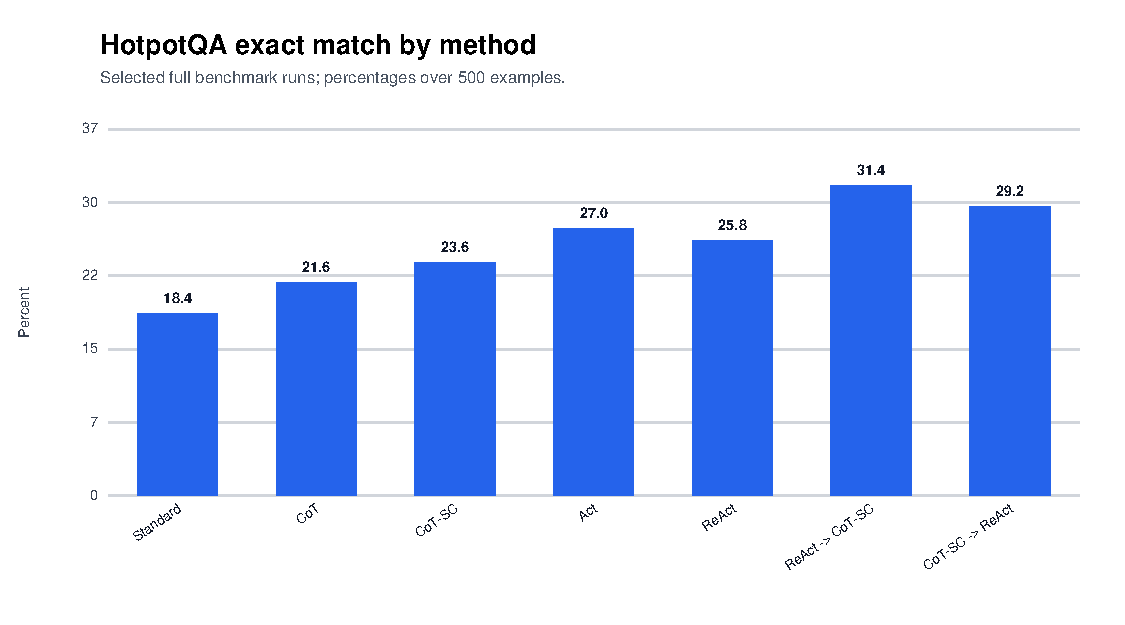
\includegraphics[width=0.92\linewidth]{figures/hotpotqa_exact_match.pdf}
\caption{HotpotQA exact match. The figure is generated from \code{results\_summary.json}.}
\label{fig:hotpot-em}
\end{figure}

ReAct $\rightarrow$ CoT-SC has the highest EM and F1. Act is the strongest single interactive strategy at 27.0 EM, slightly ahead of ReAct at 25.8. The closed-book sequence Standard, CoT, and CoT-SC improves monotonically, but each increment increases inference cost.

\subsection{Agent and Retrieval Behavior}

Standalone ReAct completes 279 trajectories, exhausts the step budget on 197, and stops on an action loop on 24. Its 129 exact matches all occur among completed trajectories, yielding 46.2\% EM within that subset. Across the run, ReAct makes 1,811 searches and 480 lookups. It records 346 Lookup misses and repeats an exact Search action in 116 examples.

ReAct $\rightarrow$ CoT-SC preserves 260 completed ReAct results, of which 122 are exact matches. Its 240 fallback examples add 35 exact matches. CoT-SC $\rightarrow$ ReAct accepts 216 initial consensus results, with 102 exact matches; ReAct completes 128 of the 284 fallback cases and answers 44 correctly, while 156 hybrid trajectories fail to produce an answer.

\subsection{Failure Analysis}

The trajectories distinguish failures to identify an entity from failures to retrieve the second-hop relation. In one successful case, ReAct opens Greyia and Calibanus, compares their reported species counts, and answers Greyia in three steps. In the Tokarev failure, the agent correctly discovers Moscow State University but cannot retrieve its founding year. Two unsuccessful lookups and three reformulated searches consume the remaining budget. This is not an answer-parser failure; it is a retrieval-control failure ending in \code{max\_steps\_exceeded}.

The run contains only two malformed standalone ReAct action steps, whereas 221 examples end through a step limit or loop. Formatting therefore has little explanatory power for the aggregate HotpotQA failure rate. The larger issue is conversion of partial evidence into an efficient second-hop query and a timely Finish action.

\section{FEVER Results}

\subsection{Main Results}

\begin{table}[htbp]
\centering
\caption{FEVER results on the selected 500-example runs.}
\label{tab:fever-main}
\small
\begin{tabular}{lrrrrrr}
\toprule
Method & Correct & Accuracy & Invalid & Steps & Tools & Runtime (min) \\
\midrule
Standard & 258 & 51.6 & 2 & 1.000 & 0.000 & 1.31 \\
CoT & 280 & 56.0 & 5 & 1.000 & 0.000 & 2.93 \\
CoT-SC & 286 & 57.2 & 0 & 21.000 & 0.000 & 62.93 \\
Act & 271 & 54.2 & 39 & 2.806 & 1.802 & 27.98 \\
ReAct & 164 & 32.8 & 258 & 4.058 & 3.432 & 79.42 \\
ReAct $\rightarrow$ CoT-SC & 308 & \textbf{61.6} & 0 & 15.064 & 3.446 & 170.95 \\
CoT-SC $\rightarrow$ ReAct & 275 & 55.0 & 15 & 21.216 & 0.190 & 118.03 \\
\bottomrule
\end{tabular}
\end{table}

\begin{figure}[htbp]
\centering
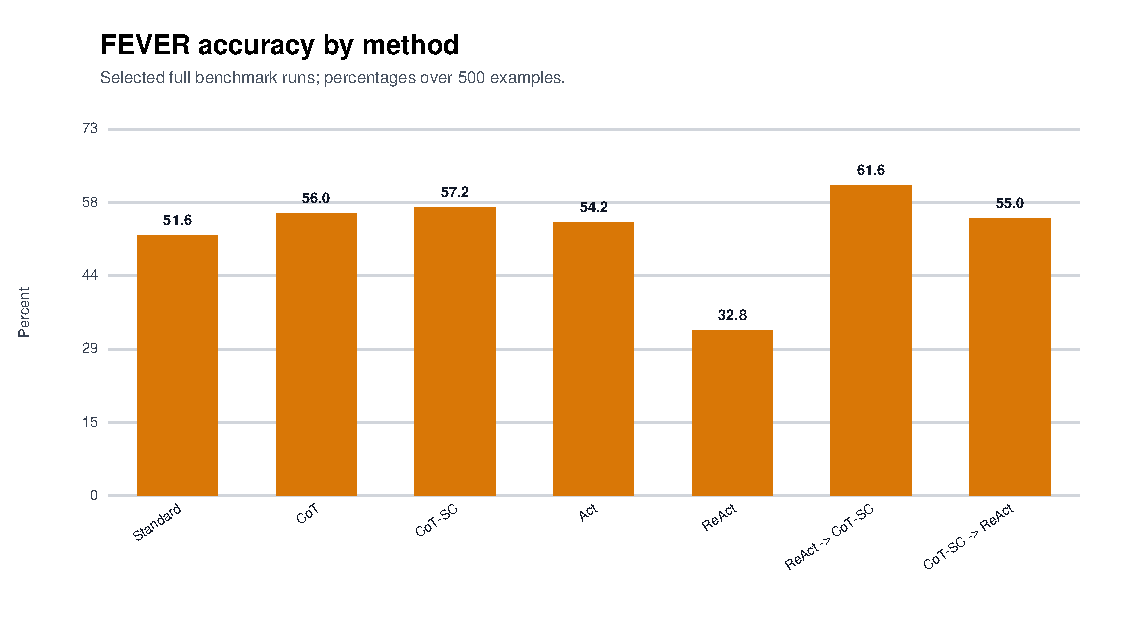
\includegraphics[width=0.92\linewidth]{figures/fever_accuracy.pdf}
\caption{FEVER label accuracy. The large standalone ReAct deficit includes non-completions.}
\label{fig:fever-accuracy}
\end{figure}

ReAct $\rightarrow$ CoT-SC reaches 61.6\% accuracy and has no invalid final predictions. CoT-SC is the strongest non-hybrid at 57.2\%. Standalone ReAct returns 258 invalid/unparsed predictions, causing its aggregate accuracy to fall to 32.8\% despite strong completed cases.

\subsection{Class-Level Analysis}

\begin{table}[htbp]
\centering
\caption{FEVER per-class accuracy (\%).}
\label{tab:fever-class}
\small
\begin{tabular}{lrrr}
\toprule
Method & Supports & Refutes & Not Enough Info \\
\midrule
Standard & 55.7 & 74.6 & 29.9 \\
CoT & 75.9 & 68.3 & 27.7 \\
CoT-SC & 78.7 & 68.3 & 28.3 \\
Act & 52.9 & 73.2 & \textbf{40.8} \\
ReAct & 37.9 & 35.9 & 25.5 \\
ReAct $\rightarrow$ CoT-SC & \textbf{78.7} & \textbf{70.4} & 38.6 \\
CoT-SC $\rightarrow$ ReAct & 75.3 & 66.9 & 26.6 \\
\bottomrule
\end{tabular}
\end{table}

Not Enough Info is the hardest class for every method. Self-consistency improves Supports but leaves NEI below 29\%. Act obtains the highest NEI accuracy, although its invalid predictions and weaker Supports performance lower its aggregate score. ReAct $\rightarrow$ CoT-SC combines strong Supports and Refutes performance with a substantial NEI improvement over standalone CoT-SC.

\subsection{Agent and Retrieval Behavior}

Standalone ReAct completes 242 examples, reaches the five-step limit on 243, and ends with a parsing error on 15. All 164 correct predictions are in the completed group, which has 67.8\% accuracy. Empty predictions from budget exhaustion must therefore be separated from malformed generations.

ReAct makes 1,705 searches, of which 1,469 receive a \code{Could not find} observation with suggestions. Only 11 Lookup actions appear. For the Peking University claim, five increasingly specific queries all return suggestions containing the exact article title, but the model never issues \code{Search[Peking University]}. The environment preserves paper-style action semantics rather than silently selecting that suggestion.

The current implementation attempts one action-only recovery when a combined Thought/Action completion cannot be parsed. The retry occurs in the same logical step, runs only for failed batch states, stops at a newline, and is subjected to deterministic truncation. The serializer stores the recovered completion rather than both generations. In standalone FEVER, 29 action-only serialized outputs are consistent with successful recovery, while 71 steps across 68 examples remain invalid after recovery. This modern batched implementation preserves the original protocol's same-step semantics but batches the recovery calls for efficiency and state isolation.

\subsection{Failure Analysis}

The artifacts expose three quantitatively important classes of standalone ReAct failure. First, 243 examples exhaust the environment budget without Finish. Second, 15 finish with \code{parsing\_error}; malformed steps can also occur earlier in trajectories that continue. Third, 78 of the 242 completed examples return a valid but wrong label, indicating evidence selection or interpretation errors. These categories should not be collapsed into a single parser-failure explanation.

Act has 39 invalid predictions, with 409 ordinary completions, 52 completions at the step limit, and 39 failed finalizations. Standard and CoT have 2 and 5 invalid labels, respectively; CoT-SC has none. The label parser is therefore not the dominant source of FEVER error outside a small number of direct-generation cases.

\section{Cross-Task Comparison}

HotpotQA and FEVER both benefit from factual knowledge, but they stress different aspects of the agent loop. HotpotQA requires open-ended answer normalization and often an explicit second hop. Its successful trajectories commonly retrieve two entities and compose a relation across them. FEVER has a small output vocabulary, but the agent must determine whether evidence entails, contradicts, or fails to resolve a claim.

This difference affects self-consistency. On FEVER, 21 generations vote over three labels and always yield a valid aggregate label in the selected run. On HotpotQA, surface variation fragments votes across many strings, and a normalized plurality can still be weak. Retrieval also behaves differently: HotpotQA Lookup is used frequently, while FEVER ReAct overwhelmingly issues Search queries and rarely follows with Lookup.

\begin{figure}[htbp]
\centering
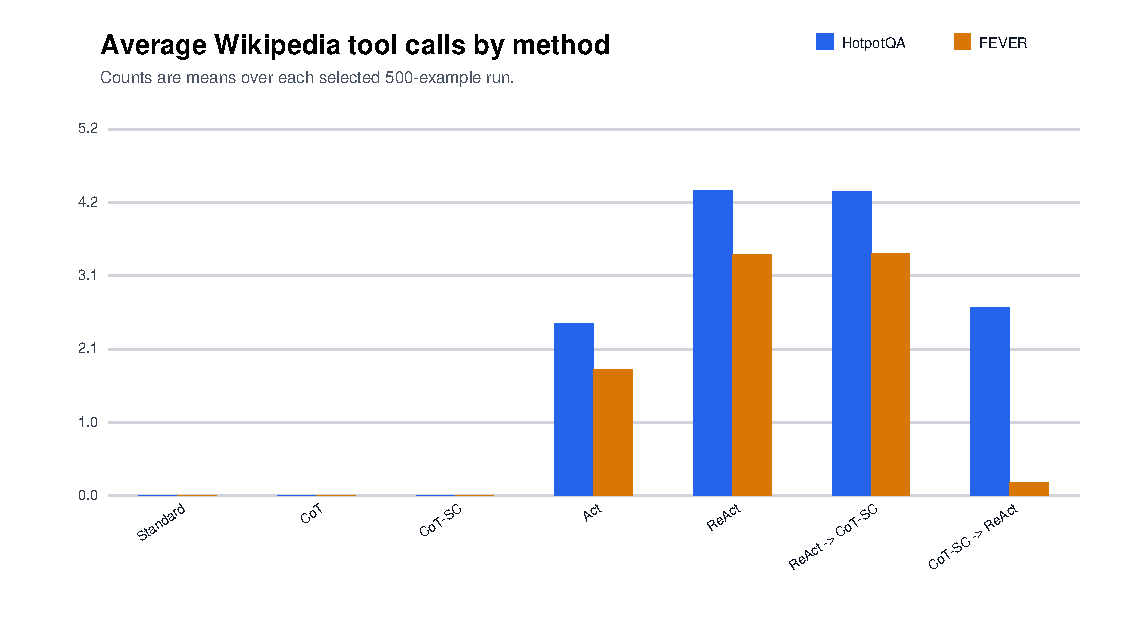
\includegraphics[width=0.92\linewidth]{figures/average_tool_calls.pdf}
\caption{Average Wikipedia tool calls. CoT-SC steps are not tool calls and are excluded from this accounting.}
\label{fig:tools}
\end{figure}

The hybrid direction is consequential on both tasks. ReAct $\rightarrow$ CoT-SC performs best overall because a completed ReAct path can be retained while the closed-book vote supplies an answer for failures. CoT-SC $\rightarrow$ ReAct uses few FEVER tools because only 25 claims fall below its confidence threshold; however, those cases are unusually difficult, and ReAct completes only 10 of them.

\section{Discussion}

\subsection{ReAct versus Non-Agentic Reasoning}

Interactive methods reduce dependence on parametric knowledge but add exposure to query formulation, environment state, and termination. On HotpotQA, Act and ReAct outperform Standard, CoT, and CoT-SC in EM. On FEVER, completed ReAct cases are accurate, but its low completion rate overwhelms that advantage. ReAct should therefore be evaluated jointly on decision quality and completion behavior.

\subsection{Effect of Self-Consistency}

CoT-SC improves over CoT by 2.0 EM points on HotpotQA and 1.2 accuracy points on FEVER. It also removes invalid FEVER labels. The gains are measurable but expensive: 21 generations per example increase runtime from 2.44 to 54.16 minutes on HotpotQA and from 2.93 to 62.93 minutes on FEVER.

\subsection{Hybrid Reasoning Strategies}

ReAct $\rightarrow$ CoT-SC improves robustness by filling in missing ReAct answers. On FEVER, its completed-ReAct path has 68.5\% accuracy across 238 examples, while the fallback path has 55.3\% across 262. CoT-SC $\rightarrow$ ReAct accepts 475 FEVER votes at 57.1\% accuracy; its 25 fallback cases yield only 4 correct labels and 15 failures. Routing is therefore not neutral: the first-stage confidence rule determines the difficulty distribution seen by the fallback.

\subsection{Accuracy versus Tool and Inference Cost}

Standard and CoT are inexpensive but less accurate. CoT-SC spends sampling compute without tools. ReAct spends environment calls and may still fail to answer. ReAct $\rightarrow$ CoT-SC has the strongest scores but the highest FEVER runtime because many examples pay for both a full ReAct attempt and 21 CoT samples. Wall-clock values remain descriptive because batch sizes differ.

\subsection{Effect of Using a Modern Instruction-Tuned Model}

Table~\ref{tab:paper-comparison} separates the original PaLM-540B values in the repository's copy of the ReAct paper from the present Qwen reproduction. The comparison is not model-controlled. It is included to locate the reproduction, not to attribute differences to a single cause.

\begin{table}[htbp]
\centering
\caption{Original-paper results and this reproduction (percentage points).}
\label{tab:paper-comparison}
\small
\begin{tabular}{lrrrr}
\toprule
& \multicolumn{2}{c}{HotpotQA EM} & \multicolumn{2}{c}{FEVER accuracy} \\
\cmidrule(lr){2-3}\cmidrule(lr){4-5}
Method & Paper & Reproduction & Paper & Reproduction \\
\midrule
Standard & 28.7 & 18.4 & 57.1 & 51.6 \\
CoT & 29.4 & 21.6 & 56.3 & 56.0 \\
CoT-SC & 33.4 & 23.6 & 60.4 & 57.2 \\
Act & 25.7 & 27.0 & 58.9 & 54.2 \\
ReAct & 27.4 & 25.8 & 60.9 & 32.8 \\
ReAct $\rightarrow$ CoT-SC & 35.1 & 31.4 & 62.0 & 61.6 \\
CoT-SC $\rightarrow$ ReAct & 34.2 & 29.2 & 64.6 & 55.0 \\
\bottomrule
\end{tabular}
\end{table}

The absolute gaps vary across methods and tasks. In particular, the FEVER standalone ReAct score is governed by completion failures specific to this model--environment interaction. At the same time, the ReAct $\rightarrow$ CoT-SC FEVER result is close to the original paper value. These observations suggest that the protocol's fallback structure transfers more reliably than every component's standalone performance.

\section{Limitations}

The experiments use 500-example seeded samples rather than complete evaluation splits, and no confidence intervals or significance tests are reported. HotpotQA methods span multiple historical code versions, and its model revision and standalone ReAct batch size are missing. Wikipedia is a live external dependency without a pinned content snapshot. Runtimes are affected by batching and hardware. HotpotQA supporting-fact metrics are unavailable because supporting facts are not predicted. Finally, the original-paper comparison changes the model, inference stack, and likely environment state, so it is descriptive rather than causal.

\section{Conclusion}

Across both tasks, ReAct $\rightarrow$ CoT-SC provides the strongest aggregate result: 31.4 EM on HotpotQA and 61.6 accuracy on FEVER. The advantage arises from complementarity. ReAct produces strong answers when it completes, while CoT-SC supplies a valid answer when interaction fails. The trajectory evidence also identifies the remaining bottleneck: retrieval access alone is insufficient when the model formulates over-specific queries, ignores useful suggestions, or does not emit a final answer before the environment budget expires.

\appendix
\section{Full Configuration}

\begin{longtable}{p{2.6cm}p{1.15cm}p{1.1cm}p{1.3cm}p{1.1cm}p{1.25cm}p{1.45cm}}
\caption{Selected-run configuration. A dash denotes a field not recorded or not applicable.}\label{tab:config}\\
\toprule
Task / method & Code & Batch & Max steps & CoT-SC $n$ & CoT-SC temp. & Best effort \\
\midrule
\endfirsthead
\toprule
Task / method & Code & Batch & Max steps & CoT-SC $n$ & CoT-SC temp. & Best effort \\
\midrule
\endhead
HotpotQA Standard & 0.10.0 & 32 & 7 & -- & -- & -- \\
HotpotQA CoT & 0.10.0 & 16 & 7 & -- & -- & -- \\
HotpotQA CoT-SC & 0.10.0 & 16 & 7 & 21 & 0.7 & -- \\
HotpotQA Act & 0.10.0 & 16 & 7 & -- & -- & -- \\
HotpotQA ReAct & 0.8.1 & -- & 7 & -- & -- & false \\
HotpotQA ReAct $\rightarrow$ CoT-SC & 0.9.0 & 8 & 7 & 21 & 0.7 & false \\
HotpotQA CoT-SC $\rightarrow$ ReAct & 0.9.0 & 3 & 7 & 21 & 0.7 & false \\
FEVER Standard & 0.11.0 & 32 & 5 & -- & -- & -- \\
FEVER CoT & 0.11.0 & 16 & 5 & -- & -- & -- \\
FEVER CoT-SC & 0.11.0 & 16 & 5 & 21 & 0.7 & -- \\
FEVER Act & 0.11.0 & 16 & 5 & -- & -- & -- \\
FEVER ReAct & 0.11.0 & 8 & 5 & -- & -- & false \\
FEVER ReAct $\rightarrow$ CoT-SC & 0.11.0 & 8 & 5 & 21 & 0.7 & false \\
FEVER CoT-SC $\rightarrow$ ReAct & 0.11.0 & 8 & 5 & 21 & 0.7 & false \\
\bottomrule
\end{longtable}

\section{Additional Metrics}

\begin{table}[htbp]
\centering
\caption{Termination and route counts used in the analysis.}
\small
\begin{tabularx}{\linewidth}{lX}
\toprule
Run & Counts \\
\midrule
HotpotQA ReAct & completed 279; max steps 197; action loop 24 \\
HotpotQA ReAct $\rightarrow$ CoT-SC & ReAct completed 260; CoT-SC fallback 240 \\
HotpotQA CoT-SC $\rightarrow$ ReAct & CoT-SC consensus 216; ReAct completed 128; failed 156 \\
FEVER ReAct & completed 242; max steps 243; parsing error 15 \\
FEVER ReAct $\rightarrow$ CoT-SC & ReAct completed 238; CoT-SC fallback 262 \\
FEVER CoT-SC $\rightarrow$ ReAct & CoT-SC consensus 475; ReAct completed 10; failed 15 \\
\bottomrule
\end{tabularx}
\end{table}

\section{Representative Trajectories}

\textbf{Successful HotpotQA multi-hop ReAct.} For the Greyia--Calibanus comparison, the abbreviated sequence is \code{Search[Greyia]} $\rightarrow$ ``three species,'' \code{Search[Calibanus]} $\rightarrow$ ``two species,'' then \code{Finish[Greyia]}.

\textbf{HotpotQA failure.} For the Tokarev question, the agent identifies Moscow State University but receives no match for two founding-year lookups. Three reformulated searches return the same lead, and step seven ends without Finish.

\textbf{Successful FEVER ReAct.} For ``Yandex is an application,'' \code{Search[Yandex]} opens an article describing a technology company and its services. The next action is \code{Finish[REFUTES]}.

\textbf{FEVER max-step failure.} For the Peking University founding-century claim, five over-specific searches fail while suggesting the exact title. ReAct never follows the suggestion and exhausts the budget.

\textbf{Hybrid fallback.} ReAct $\rightarrow$ CoT-SC applies the same five unsuccessful Peking University searches, then samples 21 CoT decisions. The vote consistently identifies 1898 as a nineteenth-century founding date and returns \textsc{Refutes}.

\begin{thebibliography}{9}
\bibitem{yao2023react}
Shunyu Yao, Jeffrey Zhao, Dian Yu, Nan Du, Izhak Shafran, Karthik Narasimhan, and Yuan Cao.
\newblock ReAct: Synergizing Reasoning and Acting in Language Models.
\newblock \emph{International Conference on Learning Representations}, 2023.

\bibitem{wei2022cot}
Jason Wei, Xuezhi Wang, Dale Schuurmans, Maarten Bosma, Fei Xia, Ed Chi, Quoc Le, and Denny Zhou.
\newblock Chain-of-Thought Prompting Elicits Reasoning in Large Language Models.
\newblock \emph{Advances in Neural Information Processing Systems}, 2022.

\bibitem{wang2023selfconsistency}
Xuezhi Wang, Jason Wei, Dale Schuurmans, Quoc Le, Ed Chi, Sharan Narang, Aakanksha Chowdhery, and Denny Zhou.
\newblock Self-Consistency Improves Chain of Thought Reasoning in Language Models.
\newblock \emph{International Conference on Learning Representations}, 2023.
\end{thebibliography}

\end{document}
